%iffalse
\let\negmedspace\undefined
\let\negthickspace\undefined
\documentclass[journal,12pt,onecolumn]{IEEEtran}
\usepackage[version=4]{mhchem}
\usepackage{chemformula} % for \ch if needed
\usepackage{chemfig}
\usepackage{chemmacros}
\chemsetup{modules = reactions} % Enables reaction arrows
\usepackage{graphicx}
\graphicspath{ {./images/} }

\usepackage{fancyhdr}
\usepackage{geometry}
\usepackage{lastpage}
\usepackage{cite}
\usepackage{amsmath,amssymb,amsfonts,amsthm}
\usepackage{enumitem,multicol}
\usepackage{algorithmic}
\usepackage{graphicx}
\usepackage{textcomp}
\usepackage{xcolor}
\usepackage{txfonts}
\usepackage{listings}
\usepackage{enumitem}
\usepackage{mathtools}
\usepackage{gensymb}
\usepackage{comment}
\usepackage[breaklinks=true]{hyperref}
\usepackage{tkz-euclide}
\usepackage{listings}
\usepackage{gvv}                                        
%\def\inputGnumericTable{}                                
\usepackage[latin1]{inputenc}                                
\usepackage{color}                                            
\usepackage{array}                                            
\usepackage{longtable}                                      
\usepackage{calc}                                            
\usepackage{multirow}                                        
\usepackage{hhline}                                          
\usepackage{ifthen}                                          
\usepackage{lscape}
\usepackage{tabularx}
\usepackage{array}
\usepackage{float}


\newtheorem{theorem}{Theorem}[section]
\newtheorem{problem}{Problem}
\newtheorem{proposition}{Proposition}[section]
\newtheorem{lemma}{Lemma}[section]
\newtheorem{corollary}[theorem]{Corollary}
\newtheorem{example}{Example}[section]
\newtheorem{definition}[problem]{Definition}
\newcommand{\BEQA}{\begin{eqnarray}}
\newcommand{\EEQA}{\end{eqnarray}}
\newcommand{\define}{\stackrel{\triangle}{=}}
\theoremstyle{remark}

\geometry{margin=1 in}

\pagestyle{fancy}
\fancyhead[L]{2011}
\fancyhead[C]{}
\fancyhead[R]{CY}
\fancyfoot[L]{CY}
\fancyfoot[C]{}
\fancyfoot[R]{\thepage/12}

\setlength{\headheight}{14pt}
\setlength{\headsep}{5pt}
\setlength{\footskip}{20pt}


% Line thickness
\renewcommand{\headrulewidth}{0.4pt}
\renewcommand{\footrulewidth}{0.4pt}



% Marks the beginning of the document
\begin{document}



\title{
GATE 2011 \\
CY: CHEMISTRY}
\author{AI25BTECH11008 - Chiruvella Harshith Sharan}
\maketitle


\begin{enumerate}


\item    Jahn-Teller distortion of CuSO$_4\cdot$5H$_2$O acts to \hfill{\brak{\textbf{GATE CY 2011}}}
 

\begin{multicols}{2}
\begin{enumerate}
\item raise symmetry  
\item remove an electronic degeneracy  
\item cause loss of H$_2$O ligand  
\item promote a d-electron to an antibonding molecular orbital  
\end{enumerate}
\end{multicols}
 

\item    Among the following, the group of molecules that undergoes rapid hydrolysis is \hfill{\brak{\textbf{GATE CY 2011}}}
 

\begin{multicols}{2}
\begin{enumerate}
\item SF$_6$, Al$_2$Cl$_6$, SiMe$_4$  
\item BCl$_3$, SF$_6$, SiCl$_4$  
\item BCl$_3$, SiCl$_4$, PCl$_5$  
\item SF$_6$, Al$_2$Cl$_6$, SiCl$_4$  
\end{enumerate}
\end{multicols}
 

\item    The reaction of solid XeF$_2$ with AsF$_5$ in 1:1 ratio affords \hfill{\brak{\textbf{GATE CY 2011}}}
 

\begin{multicols}{2}
\begin{enumerate}
\item XeF$_4$ and AsF$_3$  
\item XeF$_6$ and AsF$_3$  
\item [XeF$^+$][AsF$_6^-$]  
\item [Xe$_2$F$_3^+$][AsF$_6^-$]  
\end{enumerate}
\end{multicols}
 

\item    A well known naturally occurring organometallic compound is \hfill{\brak{\textbf{GATE CY 2011}}}
 

\begin{multicols}{2}
\begin{enumerate}
\item vitamin B$_{12}$ coenzyme  
\item chlorophyll  
\item cytochrome P-450  
\item myoglobin  
\end{enumerate}
\end{multicols}
 

\item    The complex that exists as a pair of enantiomers is \hfill{\brak{\textbf{GATE CY 2011}}}
 

\begin{multicols}{2}
\begin{enumerate}
\item trans-[Co(H$_2$NCH$_2$CH$_2$NH$_2$)$_2$Cl$_2$]$^+$  
\item cis-[Co(NH$_3$)$_4$Cl$_2$]$^+$  
\item[(C)] [Pt(PPh$_3$)(Cl)(Br)(CH$_3$)]$^-$  
\item[(D)] [Co(H$_2$NCH$_2$CH$_2$NH$_2$)$_3$]$^{3+}$  
\end{enumerate}
\end{multicols}
 

\item    The region of electromagnetic spectrum employed in the electron spin resonance (ESR) spectroscopy is \hfill{\brak{\textbf{GATE CY 2011}}}
 

\begin{multicols}{2}
\begin{enumerate}
\item radiowave  
\item microwave  
\item infrared  
\item visible  
\end{enumerate}
\end{multicols}
 

\item    The red color of oxyhaemoglobin is mainly due to the \hfill{\brak{\textbf{GATE CY 2011}}}
 

\begin{multicols}{2}
\begin{enumerate}
\item d-d transition  
\item metal to ligand charge transfer transition  
\item ligand to metal charge transfer transition  
\item intraligand $\pi$-$\pi^*$ transition  
\end{enumerate}
\end{multicols}
 

\item    The band structure in an n-type semiconductor is \hfill{\brak{\textbf{GATE CY 2011}}}
 


\begin{figure}[H][H]
    \centering
   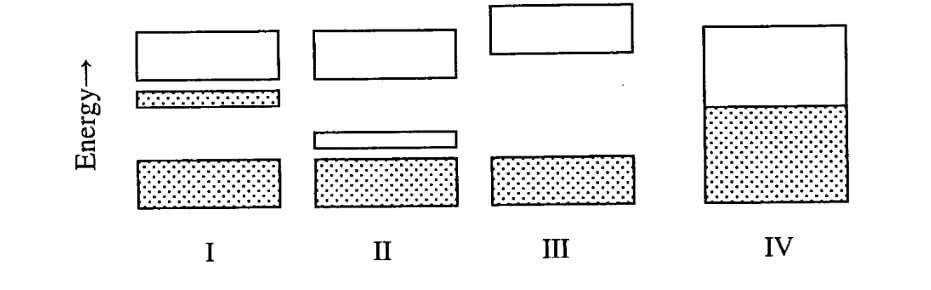
\includegraphics[width=0.6\columnwidth]{figs/image1.jpg}
      \caption{}
    \label{fig:figure1}
\end{figure}
   


\begin{multicols}{2}
\begin{enumerate}
\item I  
\item II  
\item III  
\item IV  
\end{enumerate}
\end{multicols}
 



\item    In the following reaction \hfill{\brak{\textbf{GATE CY 2011}}}
 

\begin{figure}[H][H]
    \centering
    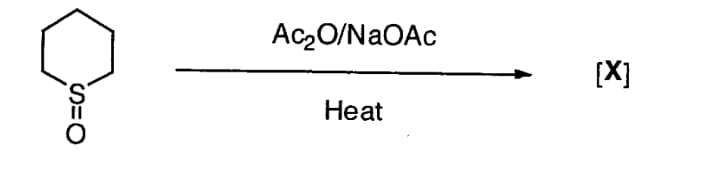
\includegraphics[width=0.5\columnwidth]{figs/image2.jpg}
    \caption{}
    \label{fig:figure2}
\end{figure}




\noindent The major product \textbf{[X]} is:
 
\begin{figure}[H][H]
    \centering
    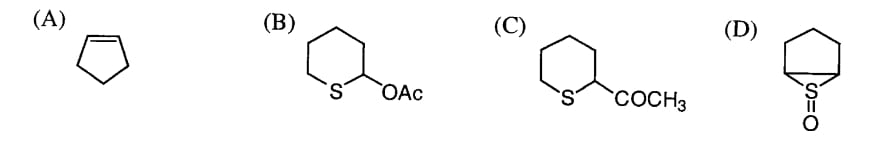
\includegraphics[width=0.8\columnwidth]{figs/image3.jpg}
    \caption{}
    \label{fig:figure3}
\end{figure}


 

\newpage
\item    In the following reaction sequence: \hfill{\brak{\textbf{GATE CY 2011}}}
 


\begin{figure}[H][H]
    \centering
    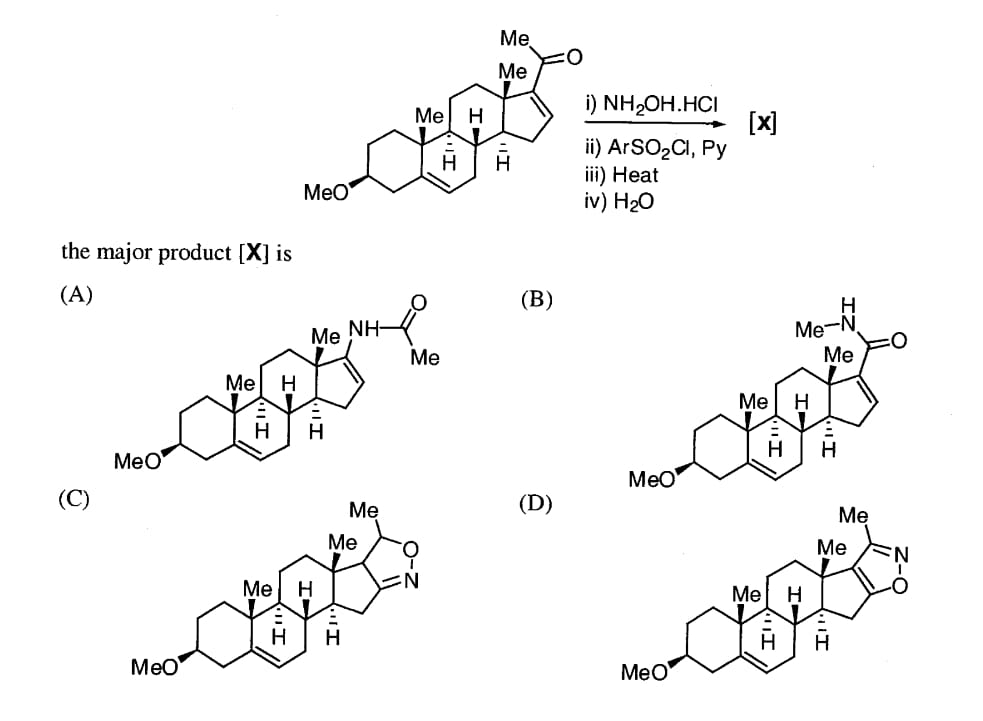
\includegraphics[width=1\columnwidth]{figs/image4.jpg}
    \caption{}
    \label{fig:figure4}
\end{figure}

 

\newpage
\

\item    \hspace{0.5cm} The sequence of an mRNA molecule produced from a DNA template strand with the composition 5'-AGCTCACACT-3' is  \hfill{\brak{\textbf{GATE CY 2011}}}

\begin{multicols}{2}
\begin{enumerate}
    \item 5'-AGGUUAGGCU-3'
    \item 5'-UCGAUGUGA-3'
    \item 5'-AGTGTAGCT-3'
    \item 5'-TCGATGTGA-3'
\end{enumerate}
\end{multicols}
 




\item    \hspace{0.5cm} For a given first order reaction, the reactant reduces to 1/4\textsuperscript{th} its initial value in 10 minutes. The rate constant of the reaction is  \hfill{\brak{\textbf{GATE CY 2011}}}

\begin{multicols}{2}
\begin{enumerate}
    \item 0.1386 min$^{-1}$
    \item 0.0693 min$^{-1}$
    \item 0.1386 mol L$^{-1}$ min$^{-1}$
    \item 0.0693 mol L$^{-1}$ min$^{-1}$
\end{enumerate}
\end{multicols}
 

\item    \hspace{0.5cm} The freezing point constant for water is 1.86 K (mol kg$^{-1}$)$^{-1}$. The change in freezing point when 0.01 mol glucose is added to 1 kg water is  \hfill{\brak{\textbf{GATE CY 2011}}}

\begin{multicols}{2}
\begin{enumerate}
    \item 1.86 K
    \item --1.86 K
    \item 0.186 K
    \item --0.0186 K
\end{enumerate}
\end{multicols}
 

\item    \hspace{0.5cm} On the pressure-temperature diagram for a one-component system, the point where the solid-liquid and the liquid-gas curves intersect is  \hfill{\brak{\textbf{GATE CY 2011}}}

\begin{multicols}{2}
\begin{enumerate}
    \item triple point
    \item critical point
    \item melting point
    \item boiling point
\end{enumerate}
\end{multicols}

 
\item    \hspace{0.5cm} The wave function for a Harmonic oscillator described by $Nx \exp(-\alpha x^2 / 2)$ has  \hfill{\brak{\textbf{GATE CY 2011}}}

\begin{multicols}{2}
\begin{enumerate}
    \item one maximum only
    \item one maximum, one minimum only
    \item two maxima, one minimum only
    \item two maxima, two minima only
\end{enumerate}
\end{multicols}
 


\item    \hspace{0.5 cm} If an arbitrary wave function is used to calculate the energy of a quantum mechanical system, the value calculated is never less than the true energy.

The above statement relates to  \hfill{\brak{\textbf{GATE CY 2011}}}

\begin{multicols}{2}
\begin{enumerate}
    \item perturbation theory
    \item variation principle
    \item Heisenberg's uncertainty principle
    \item quantization of energy
\end{enumerate}
\end{multicols}
 

\item    \hspace{0.5 cm} The point group symmetry of the given planar shape is  \hfill{\brak{\textbf{GATE CY 2011}}}

\begin{center}
\begin{tikzpicture}[scale=1]
  % Draw central vertical line
  \draw[thick] (0,0) -- (0,1.5);
  % Draw right arm
  \draw[thick] (0,0.5) -- (1,1);
  \draw[thick] (1,1) -- (1.5,1.5);
  % Draw left arm
  \draw[thick] (0,0.5) -- (-1,1);
  \draw[thick] (-1,1) -- (-1.5,1.5);
\end{tikzpicture}
\end{center}

\begin{multicols}{2}
\begin{enumerate}
    \item D$_{3h}$
    \item C$_1$
    \item C$_{3h}$
    \item C$_{3v}$
\end{enumerate}
\end{multicols}
 

\item    \hspace{0.5cm} \( \left( \frac{\partial G}{\partial P} \right)_T = \)  \hfill{\brak{\textbf{GATE CY 2011}}}

\begin{multicols}{2}
\begin{enumerate}
    \item V
    \item S
    \item $-S$
    \item $-V$
\end{enumerate}
\end{multicols}
 


\item    \hspace{0.5cm}  \hfill{\brak{\textbf{GATE CY 2011}}}

\begin{center}
\begin{tikzpicture}[scale=1.1]
    % Axes
    \draw[->] (0,0) -- (4.2,0) node[below] {Temperature $\rightarrow$};
    \draw[->] (0,0) -- (0,3.2) node[above] {Volume $\uparrow$};

    % Transition lines
    \draw[thick] (0.5,0.5) -- (1.9,1.5);
    \draw[thick] (2.3,2.0) -- (3.8,2.8);
    \draw[dashed] (2.1,0) -- (2.1,3);

\end{tikzpicture}
\end{center}

According to the Ehrenfest classification of phase transitions, the above diagram refers to

\begin{multicols}{2}
\begin{enumerate}
    \item Zeroth order phase transition
    \item First order phase transition
    \item Second order phase transition
    \item $\lambda$ transition
\end{enumerate}
\end{multicols}
 

\item    \hspace{0.5cm} According to conventional transition state theory, for elementary bimolecular reactions, the molar entropy of activation $\Delta S^{0\ddagger}$ is  \hfill{\brak{\textbf{GATE CY 2011}}}

\begin{multicols}{2}
\begin{enumerate}
    \item positive
    \item zero
    \item negative
    \item positive for endothermic and negative for exothermic reactions
\end{enumerate}
\end{multicols}


\item    \hspace{0.5cm} The crystal field stabilization energy (CFSE) value for [Ti(H$_2$O)$_6$]$^{3+}$ that has an absorption maximum at 492 nm is  \hfill{\brak{\textbf{GATE CY 2011}}}

\begin{multicols}{2}
\begin{enumerate}
    \item 20,325 cm$^{-1}$
    \item 12,195 cm$^{-1}$
    \item 10,162 cm$^{-1}$
    \item 8,130 cm$^{-1}$
\end{enumerate}
\end{multicols}
 

\item    \hspace{0.5cm} For Et$_2$AlX (X = PPh$_2$, Ph$^-$, Cl$^-$ and F$^-$), the tendency towards dimeric structure follows the order  \hfill{\brak{\textbf{GATE CY 2011}}}

\begin{multicols}{2}
\begin{enumerate}
    \item PPh$_2$ $>$ Cl$^-$ $>$ H$^-$ $>$ Ph$^-$
    \item Cl$^-$ $>$ PPh$_2$ $>$ H$^-$ $>$ Ph$^-$
    \item Ph$^-$ $>$ H$^-$ $>$ Cl$^-$ $>$ PPh$_2$
    \item H$^-$ $>$ Ph$^-$ $>$ PPh$_2$ $>$ Cl$^-$
\end{enumerate}
\end{multicols}
 

\item    \hspace{0.5 cm} In the isoelectronic series, VO$_4^{3-}$, CrO$_4^{2-}$ and MnO$_4^-$, all members have intense charge transfer (CT) transitions. The \textbf{INCORRECT} statement is  \hfill{\brak{\textbf{GATE CY 2011}}}

\begin{multicols}{2}
\begin{enumerate}
    \item CT transitions are attributed to excitations of electrons from ligand ($\sigma$) to metal (e)
    \item MnO$_4^-$ exhibits charge transfer at shortest wavelength among the three
    \item The wavelengths of transitions increase in the order VO$_4^{3-}$ $<$ CrO$_4^{2-}$ $<$ MnO$_4^-$
    \item The charge on metal nucleus increases in the order VO$_4^{3-}$ $<$ CrO$_4^{2-}$ $<$ MnO$_4^-$
\end{enumerate}
\end{multicols}
 

\item    \hspace{0.5cm} The increasing order of wavelength of absorption for the complex ions:  
i) [Cr(NH$_3$)$_6$]$^{3+}$, ii) [CrCl$_6$]$^{3-}$, iii) [Cr(H$_2$O)$_6$]$^{3+}$, iv) [Cr(CN)$_6$]$^{3-}$, is  \hfill{\brak{\textbf{GATE CY 2011}}}

\begin{multicols}{2}
\begin{enumerate}
    \item i $<$ ii $<$ i $<$ iii
    \item iv $<$ iii $<$ i $<$ ii
    \item iv $<$ i $<$ iii $<$ ii
    \item ii $<$ i $<$ iv $<$ iii
\end{enumerate}
\end{multicols}
 

\item    \hspace{0.5cm} The total number of metal-metal bonds in Ru$_3$(CO)$_{12}$ and Co$_4$(CO)$_{12}$ respectively, is  \hfill{\brak{\textbf{GATE CY 2011}}}

\begin{multicols}{2}
\begin{enumerate}
    \item 3 and 6
    \item 4 and 5
    \item zero and 4
    \item 3 and 4
\end{enumerate}
\end{multicols}

\item    \hspace{0.5cm} According to VSEPR theory the shapes of [SF$_2$Cl$_2$] and [SO$_4$]$^{2-}$ should be  \hfill{\brak{\textbf{GATE CY 2011}}}

\begin{multicols}{2}
\begin{enumerate}
    \item trigonal planar for [SO$_4$]$^{2-}$ and trigonal pyramidal for [SF$_2$Cl$_2$]
    \item both trigonal planar
    \item trigonal pyramidal for [SO$_4$]$^{2-}$ and trigonal planar for [SF$_2$Cl$_2$]
    \item both trigonal pyramidal
\end{enumerate}
\end{multicols}

\item    \hspace{0.5cm} The product of the reaction between CH$_3$Mn(CO)$_5$ and $^{13}$CO is  \hfill{\brak{\textbf{GATE CY 2011}}}

\begin{multicols}{2}
\begin{enumerate}
    \item (CH$_3$)$^{13}$COMn(CO)$_5$
    \item (CH$_3$)COMn(CO)$_4$($^{13}$CO)
    \item (CH$_3$)COMn($^{13}$CO)$_5$
    \item (CH$_3$)$^{13}$COMn($^{13}$CO)$_4$(CO)
\end{enumerate}
\end{multicols}
 

\item    \hspace{0.5cm} The $^1$H and $^{31}$P NMR spectra of (CH$_3$)$_2$N(CH$_2$)PPh$_2$ and (CH$_3$)$_2$N(CH$_2$)P(Cl)$_2$ is  \hfill{\brak{\textbf{GATE CY 2011}}}

\begin{figure}[H][H]
    \centering
    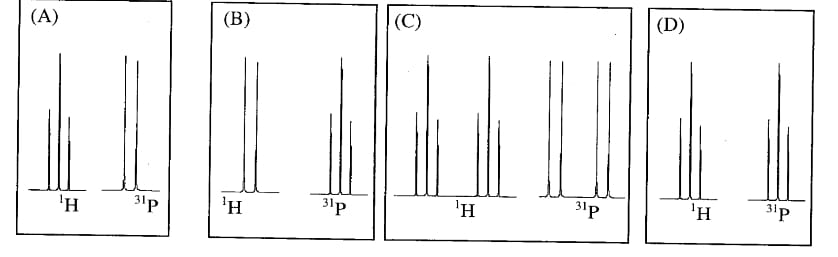
\includegraphics[width=\linewidth]{figs/image5.jpg}
    \caption{}
    \label{fig:figure11}
\end{figure}
 

\item    \hspace{0.5cm} In the following reaction  \hfill{\brak{\textbf{GATE CY 2011}}}

\begin{figure}[H][H]
    \centering
    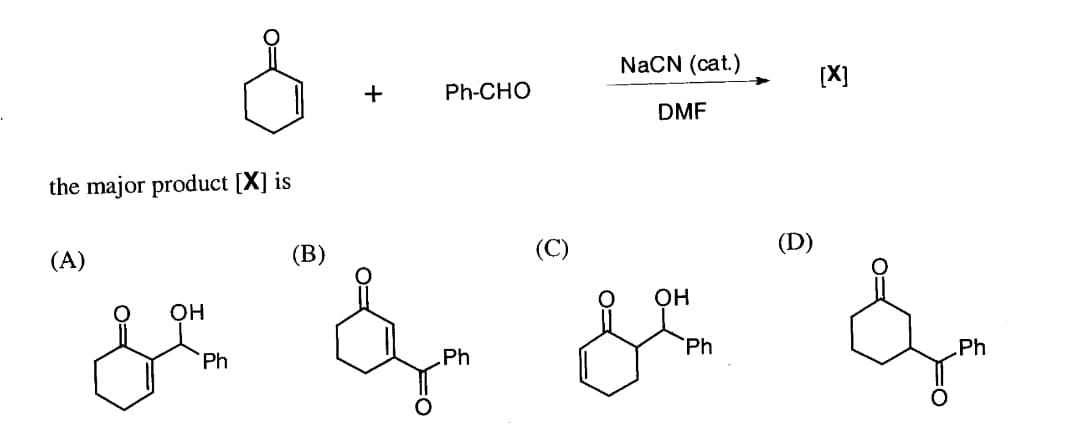
\includegraphics[width=\textwidth]{figs/image6.jpg}
    \caption{}
    \label{fig:figure6}
\end{figure}


\item    \hspace{0.5cm} The most appropriate sequence of reactions for carrying out the following conversion is  \hfill{\brak{\textbf{GATE CY 2011}}}

\begin{figure}[H]
    \centering
    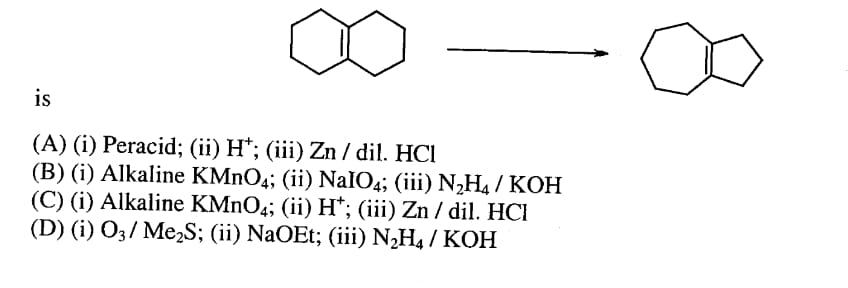
\includegraphics[width=\textwidth]{figs/image7.jpg}
    \caption{}
    \label{fig:figure7}
\end{figure}

\begin{multicols}{2}
\begin{enumerate}
    \item Peracid; (ii) H$^+$; (iii) Zn / dil. HCl
    \item (i) Alkaline KMnO$_4$; (ii) NaIO$_4$; (iii) N$_2$H$_4$/KOH
    \item (i) Alkaline KMnO$_4$; (ii) H$^+$; (iii) Zn / dil. HCl
    \item (i) O$_3$ / Me$_2$S; (ii) NaOEt; (iii) N$_2$H$_4$/KOH
\end{enumerate}
\end{multicols}




 

\item    \hspace{0.5cm} In the reaction  \hfill{\brak{\textbf{GATE CY 2011}}}

\begin{center}
\noindent Optically pure (+)-\textit{trans}-2-acetoxycyclohexyl tosylate
\[
\ce{->[\ce{HOAc}, \ce{KOAc}][\Delta]}[\textbf{X}]
\]
\end{center}

The major product [X] is:

\begin{multicols}{2}
\begin{enumerate}
    \item racemic trans-1,2-cyclohexanediol diacetate
    \item optically active trans-1,2-cyclohexanediol diacetate
    \item racemic cis-1,2-cyclohexanediol diacetate
    \item optically active cis-1,2-cyclohexanediol diacetate
\end{enumerate}
\end{multicols}

 

\item    \hspace{0.5 cm} The activity of water at 11 bar and 298 K is  \hfill{\brak{\textbf{GATE CY 2011}}}

\begin{multicols}{2}
\begin{enumerate}
    \item 1.101
    \item 1.007
    \item 0.998
    \item 0.898
\end{enumerate}
\end{multicols}

 

\item    \hspace{0.5 cm} For the process  \hfill{\brak{\textbf{GATE CY 2011}}}

\begin{center}
\textbf{1 Ar (300 K, 1 bar) $\rightarrow$ 1 Ar (200 K, 10 bar)}
\end{center}

Assuming ideal gas behavior, the change in molar entropy is:

\begin{multicols}{2}
\begin{enumerate}
    \item $-27.57 \ \text{J K}^{-1} \text{mol}^{-1}$
    \item $+27.57 \ \text{J K}^{-1} \text{mol}^{-1}$
    \item $-24.20 \ \text{J K}^{-1} \text{mol}^{-1}$
    \item $+24.20 \ \text{J K}^{-1} \text{mol}^{-1}$
\end{enumerate}
\end{multicols}

 

\item    \hspace{0.5 cm} The wave function for a quantum mechanical particle in a 1-dimensional box of length 'a' is given by  \hfill{\brak{\textbf{GATE CY 2011}}}

\[
\psi = A \sin\left(\frac{\pi x}{a}\right)
\]

The value of 'A' for a box of length 200 nm is:

\begin{multicols}{2}
\begin{enumerate}
    \item $4 \times 10^4 \ (\text{nm})^{1/2}$
    \item $10\sqrt{2} \ (\text{nm})^{1/2}$
    \item $\frac{\sqrt{2}}{10} \ (\text{nm})^{-1/2}$
    \item $0.1 \ (\text{nm})^{-1/2}$
\end{enumerate}
\end{multicols}

\item    \hspace{0.5cm} For 1 mole of a monoatomic ideal gas, the relation between pressure (\(p\)), volume (\(V\)) and average molecular kinetic energy (\(\bar{E}\)) is  \hfill{\brak{\textbf{GATE CY 2011}}}

\begin{multicols}{2}
\begin{enumerate}
    \item \(p = \dfrac{N_A \bar{E}}{V}\)
    \item \(p = \dfrac{N_A \bar{E}}{3V}\)
    \item \(p = \dfrac{2 N_A \bar{E}}{3V}\)
    \item \(p = \dfrac{2 N_A}{3V} \bar{E}\)
\end{enumerate}
\end{multicols}

 

\item    \hspace{0.5cm} For a 1 molal aqueous NaCl solution, the mean ionic activity coefficient (\(\gamma_{\pm}\)) and the Debye-Hückel Limiting Law constant (A) are related as  \hfill{\brak{\textbf{GATE CY 2011}}}

\begin{multicols}{2}
\begin{enumerate}
    \item \(\log \gamma_{\pm} = \sqrt{2} A\)
    \item \(\log \gamma_{\pm} = - \sqrt{2} A\)
    \item \(\gamma_{\pm} = 10^A\)
    \item \(\gamma_{\pm} = 10^{-A}\)
\end{enumerate}
\end{multicols}

 

\item    \hspace{0.5cm} For the concentration cell\\
\centerline{M $\vert$ M\textsuperscript{n+}(aq, 0.01 mol dm\textsuperscript{-3}) $\Vert$ M\textsuperscript{n+}(aq, 0.1 mol dm\textsuperscript{-3}) $\vert$ M}\\
The EMF (E) of the cell at a temperature (T) equals  \hfill{\brak{\textbf{GATE CY 2011}}}

\begin{multicols}{2}
\begin{enumerate}
    \item \(2.303 \dfrac{RT}{F}\)
    \item \(-2.303 \dfrac{RT}{F}\)
    \item \(E^\circ_{\text{M}^{n+}/\text{M}} + 2.303 \dfrac{RT}{F}\)
    \item \(E^\circ_{\text{M}^{n+}/\text{M}} - 2.303 \dfrac{RT}{F}\)
\end{enumerate}
\end{multicols}

 

% Common Data block
\noindent\textbf{Common Data for Questions 48 and 49:}\\
A hypothetical molecule XY has the following properties:

Reduced mass: \(2 \times 10^{-26}\) kg\\
X-Y bond length: 100 pm\\
Force constant of the bond: \(8 \times 10^2\) N·m\(^{-1}\)

 

\item    \hspace{0.5cm} The frequency of radiation (in cm\(^{-1}\) units) required to vibrationally excite the molecule from \(v = 0\) to \(v = 1\) state is  \hfill{\brak{\textbf{GATE CY 2011}}}

\begin{multicols}{2}
\begin{enumerate}
    \item 3184.8
    \item 2123.2
    \item 1061.6
    \item 840.0
\end{enumerate}
\end{multicols}

 
\item    \hspace{0.5cm} The frequency of radiation (in cm\(^{-1}\) units) required to rotationally excite the molecule from \(J = 0\) to \(J = 1\) state is  \hfill{\brak{\textbf{GATE CY 2011}}}

\begin{multicols}{2}
\begin{enumerate}
    \item 1.4
    \item 2.8
    \item 3.2
    \item 3.6
\end{enumerate}
\end{multicols}

 

% Common Data block
\noindent\textbf{Common Data for Questions 50 and 51:}\\
Na\(_2\)HPO\(_4\) and NaH\(_2\)PO\(_4\), on heating at high temperature produce a chain sodium pentaphosphate quantitatively.

 

\item    \hspace{0.5cm} The ideal molar ratio of Na\(_2\)HPO\(_4\) to NaH\(_2\)PO\(_4\) is  \hfill{\brak{\textbf{GATE CY 2011}}}

\begin{multicols}{2}
\begin{enumerate}
    \item 4:1
    \item 1:4
    \item 3:2
    \item 2:3
\end{enumerate}
\end{multicols}

 

\item    \hspace{0.5cm} The total charge on pentaphosphate anion is  \hfill{\brak{\textbf{GATE CY 2011}}}

\begin{multicols}{2}
\begin{enumerate}
    \item $-5$
    \item $-3$
    \item $-7$
    \item $-9$
\end{enumerate}
\end{multicols}
 



\noindent\textbf{Linked Answer Questions}
 
\noindent\textbf{Statement for Linked Answer Questions 52 and 53:}
 \\
The decomposition of ozone to oxygen \( \text{O}_2 (g) \rightarrow 3\text{O}_2(g) \) occurs by the mechanism:

\begin{align*}
&\text{(i)} \quad \text{M(g)} + \text{O}_3 (g) \xrightarrow{k_1} \text{O}_2 (g) + \text{O(g)} + \text{M(g)} \quad E_{a,1} \\
&\text{(ii)} \quad \text{O}_2 (g) + \text{O(g)} + \text{M(g)} \xrightarrow{k_2} \text{M(g)} + \text{O}_3 (g) \quad E_{a,2} \\
&\text{(iii)} \quad \text{O(g)} + \text{O}_3 (g) \xrightarrow{k_3} 2\text{O}_2 (g) \quad E_{a,3}
\end{align*}

where, M is the catalyst molecule.\\
\(k_i\) are rate constants and \(E_{a,i}\)'s are the activation energies for the elementary steps.

 \newpage

\item    \hspace{0.5cm} Under the steady state approximation for the intermediates, the rate of decomposition of ozone, \( -\dfrac{d[\text{O}_3]}{dt} \), is  \hfill{\brak{\textbf{GATE CY 2011}}}

\begin{multicols}{2}
\begin{enumerate}
    \item \( \dfrac{2k_1k_3[\text{O}_3]^2[\text{M}]}{k_2[\text{O}_2][\text{M}] + k_3[\text{O}_3]} \)
    \item \( \dfrac{2k_1k_3[\text{O}_3]^2[\text{M}]}{k_2[\text{O}_2][\text{M}] - k_3[\text{O}_3]} \)
    \item \( \dfrac{2k_2k_1[\text{O}_3][\text{M}]}{k_2[\text{O}_2][\text{M}] + k_3[\text{O}_3]} \)
    \item \( \dfrac{2k_2k_1[\text{O}_3][\text{M}]}{k_2[\text{O}_2][\text{M}] - k_3[\text{O}_3]} \)
\end{enumerate}
\end{multicols}

 

\item    \hspace{0.5cm} Assuming \(k_3[\text{O}_3] \gg k_2[\text{O}_2][\text{M}]\), the activation energy of the overall reaction is  \hfill{\brak{\textbf{GATE CY 2011}}}

\begin{multicols}{2}
\begin{enumerate}
    \item \( \dfrac{E_{a,1}E_{a,3}}{E_{a,2}} \)
    \item \( E_{a,3} + E_{a,1} - E_{a,2} \)
    \item \( E_{a,2} \)
    \item \( E_{a,1} \)
\end{enumerate}
\end{multicols}

 

\noindent\textbf{Statement for Linked Answer Questions 54 and 55:}

A ketone on treatment with bromine in methanol gives the corresponding monobromo compound [X] having molecular formula C\(_5\)H\(_9\)BrO. The compound [X] when treated with NaOMe in MeOH produces [Y] as the major product. The spectral data for compound [X] are: \( ^1\text{H NMR}: \delta 1.17 \text{(d, 6H)}, 3.02 \text{(m, 1H)}, 4.10 \text{(s, 2H)} \); \(^{13}\text{C NMR}: \delta 17, 37, 39, 210 \).



\noindent\textbf{General Aptitude (GA) Questions}



 

\item    \hspace{0.5cm} The question below consists of a pair of related words followed by four pairs of words. Select the pair that best expresses the relation in the original pair:\\
\textbf{Gladiator : Arena}  \hfill{\brak{\textbf{GATE CY 2011}}}

\begin{multicols}{2}
\begin{enumerate}
    \item dancer : stage
    \item commuter : train
    \item teacher : classroom
    \item lawyer : courtroom
\end{enumerate}
\end{multicols}

 

\item    \hspace{0.5cm} Choose the most appropriate word from the options given below to complete the following sentence:\\
\textit{Under ethical guidelines recently adopted by the Indian Medical Association, human genes are to be manipulated only to correct diseases for which \rule{2cm}{0.15mm} treatments are unsatisfactory.}  \hfill{\brak{\textbf{GATE CY 2011}}}

\begin{multicols}{2}
\begin{enumerate}
    \item similar
    \item most
    \item uncommon
    \item available
\end{enumerate}
\end{multicols}

 

\item    \hspace{0.5cm} Choose the word from the options given below that is most nearly opposite in meaning to the given word:\\
\textbf{Frequency}  \hfill{\brak{\textbf{GATE CY 2011}}}

\begin{multicols}{2}
\begin{enumerate}
    \item periodicity
    \item rarity
    \item gradualness
    \item persistency
\end{enumerate}
\end{multicols}

 

\item    \hspace{0.5cm} Choose the most appropriate word from the options given below to complete the following sentence:\\
\textit{It was her view that the country's problems had been \rule{2cm}{0.15mm} by foreign technocrats, so that to invite them to come back would be counter-productive.}  \hfill{\brak{\textbf{GATE CY 2011}}}

\begin{multicols}{2}
\begin{enumerate}
    \item identified
    \item ascertained
    \item exacerbated
    \item analysed
\end{enumerate}
\end{multicols}

 


\item    \hspace{0.5cm} There are two candidates P and Q in an election. During the campaign, 40\% of the voters promised to vote for P, and rest for Q. However, on the day of election 15\% of the voters went back on their promise to vote for P and instead voted for Q. 25\% of the voters went back on their promise to vote for Q and instead voted for P. Suppose, P lost by 2 votes, then what was the total number of voters?  \hfill{\brak{\textbf{GATE CY 2011}}}

\begin{multicols}{2}
\begin{enumerate}
    \item 100
    \item 110
    \item 90
    \item 95
\end{enumerate}
\end{multicols}

 



 

\item    \hspace{0.5cm} \textit{The horses may be able to look unhurt but very important role in the field of medicine. Horses were injected with toxins of diseases until their blood built up immunities. Then a serum was made from their blood. Serum to fight with diphtheria and tetanus were developed this way.}

It can be inferred from the passage, that horses were  \hfill{\brak{\textbf{GATE CY 2011}}}

\begin{multicols}{2}
\begin{enumerate}
    \item identified as a disease carrier
    \item given immunity to fatal diseases
    \item given diphtheria and tetanus
    \item vaccinated successfully
\end{enumerate}
\end{multicols}
 

\item    \hspace{0.5cm} The sum of $n$ terms of the series $4+44+444+\ldots$ is  \hfill{\brak{\textbf{GATE CY 2011}}}

\begin{multicols}{2}
\begin{enumerate}
    \item $\frac{4}{81} \left[10^{n+1} - 9n - 1 \right]$
    \item $\frac{4}{81} \left[10^{n} - 9n - 1 \right]$
    \item $\frac{4}{81} \left[10^{n+1} - 9n - 10 \right]$
    \item $\frac{4}{81} \left[10^n - 9n - 10 \right]$
\end{enumerate}
\end{multicols}

 

\item    \hspace{0.5cm} Given that $f(y) = \left\lfloor \frac{y}{y} \right\rfloor$, and $q$ is any non-zero real number, the value of $|f(q) - f(-q)|$ is  \hfill{\brak{\textbf{GATE CY 2011}}}

\begin{multicols}{2}
\begin{enumerate}
    \item 0
    \item -1
    \item 1
    \item 2
\end{enumerate}
\end{multicols}

 

\item    \hspace{0.5cm} Three friends, R, S and T shared toffee from a bowl. R took $\frac{1}{3}$rd of the toffees, but returned four to the bowl. S took $\frac{1}{4}$th of what was left but returned three to the bowl. T took half of the remainder but returned two back into the bowl. If the bowl had 17 toffees left, how many toffees were originally there in the bowl?  \hfill{\brak{\textbf{GATE CY 2011}}}

\begin{multicols}{2}
\begin{enumerate}
    \item 38
    \item 31
    \item 48
    \item 41
\end{enumerate}
\end{multicols}

 

\item    \hspace{0.5cm} The fuel consumed by a motorcycle during a journey while traveling at various speeds is indicated in the graph below:  \hfill{\brak{\textbf{GATE CY 2011}}}

 
 

The distances covered during four laps of the journey are listed in the table below:

 
\begin{center}
\begin{tabular}{|c|c|c|}
\hline
\textbf{Lap} & \textbf{Distance (kilometres)} & \textbf{Average speed (km/h)} \\
\hline
P & 15 & 15 \\
Q & 75 & 45 \\
R & 40 & 75 \\
S & 10 & 10 \\
\hline
\end{tabular}
\end{center}

 
From the given data, we can conclude that the fuel consumed per kilometre was least during the lap:

\begin{multicols}{2}
\begin{enumerate}
    \item P
    \item Q
    \item R
    \item S
\end{enumerate}
\end{multicols}

 

\centerline{\textbf{END OF THE QUESTION PAPER}}


\end{enumerate}



\end{document}
